%% Dokumen Uji Perangkat Lunak (DUPL)
%% Compile with: xelatex DUPL.tex

\documentclass[12pt, a4paper]{article}
% ── Simbol Tambahan ──────────────────────────────────────────────────
\usepackage{amsmath}
\usepackage{amssymb}
% ── Font & encoding ──────────────────────────────────────────────────
\usepackage{fontspec}
\setmainfont{Times New Roman}

% ── Bahasa & microtypografi ──────────────────────────────────────────
\usepackage[indonesian]{babel}
\usepackage{microtype}

% ── Layout ───────────────────────────────────────────────────────────
\usepackage[top=2.5cm, bottom=2.5cm, left=3cm, right=2.5cm]{geometry}
\usepackage{parskip}          % spasi antar paragraf, tanpa indentasi
\setlength{\parindent}{0pt}

% ── Tabel ────────────────────────────────────────────────────────────
\usepackage{booktabs}
\usepackage{tabularx}
\usepackage{longtable}
\usepackage{array}
\usepackage{multirow}
\usepackage{makecell}
\usepackage{float}
\renewcommand{\arraystretch}{1.3}

% ── Heading ──────────────────────────────────────────────────────────
\usepackage{titlesec}
\titleformat{\section}{\large\bfseries}{\thesection}{1em}{}
\titleformat{\subsection}{\normalsize\bfseries}{\thesubsection}{1em}{}
\titleformat{\subsubsection}{\normalsize\bfseries}{\thesubsubsection}{1em}{}

% ── Daftar Isi ───────────────────────────────────────────────────────
\usepackage{tocloft}
\renewcommand{\cftsecleader}{\cftdotfill{\cftdotsep}}

% ── Hyperlink ────────────────────────────────────────────────────────
\usepackage[colorlinks=true, linkcolor=black, urlcolor=blue]{hyperref}

% ── Lainnya ──────────────────────────────────────────────────────────
\usepackage{enumitem}
\usepackage{graphicx}
\usepackage{xcolor}

% ─────────────────────────────────────────────────────────────────────
\begin{document}

% ══════════════════════════════════════════════════════════════════════
%   HALAMAN JUDUL
% ══════════════════════════════════════════════════════════════════════
% ══════════════════════════════════════════════════════════════════════
%   HALAMAN JUDUL
% ══════════════════════════════════════════════════════════════════════
\begin{titlepage}
  \centering
  \vspace*{1cm}
  
  % Masukkan Logo Telkom University di bagian atas
  % Sesuaikan width (lebar) sesuai kebutuhan, misal 4cm atau 5cm
  
\includegraphics[width=4.5cm]{telkom.png}\par
  \vspace{1.5cm}
  
  {\LARGE\bfseries DOKUMEN UJI PERANGKAT LUNAK\par}
  \vspace{1cm}
  {\large \textit{Aplikasi Obibi: Pengingat Jadwal Obat Pintar}\par}
  \vspace{2.5cm} % Jarak disesuaikan setelah menghapus bagian "untuk"
  
  {\normalsize\bfseries Dipersiapkan oleh:\par}
  \vspace{0.5cm}
  {\normalsize
    Najla Tsabita Afiyah (103012400305)\\[4pt]
    Revalina Rasyidin (103012400156)\\[4pt]
    Ravi Adi Prakoso (103012430058)\\[4pt]
    Muhammad Ahsan Raziq Sulthany (103012430067)\par
  }
  \vspace{1.5cm}
  {\normalsize
    Program Studi S1 Informatika\\
    Fakultas Informatika\\
    Universitas Telkom\\[4pt]
    2026\par
  }
  \vfill
\end{titlepage}

% ══════════════════════════════════════════════════════════════════════
%   DAFTAR ISI / GAMBAR / TABEL / LAMPIRAN
% ══════════════════════════════════════════════════════════════════════
\tableofcontents
\newpage

% ══════════════════════════════════════════════════════════════════════
%   1. PENDAHULUAN
% ══════════════════════════════════════════════════════════════════════
\section{Pendahuluan}

\subsection{Tujuan Pembuatan Dokumen}

Dokumen Uji Perangkat Lunak (DUPL) ini disusun untuk mengidentifikasi produk,
mendokumentasikan skenario pengujian, serta menyajikan persyaratan kualitas dari
sistem aplikasi Obibi. Dokumen ini mendefinisikan Obibi sebagai sebuah platform
asisten kesehatan inklusif berbasis \textit{Agentic AI} dan \textit{GraphRAG}
yang dirancang secara khusus untuk membantu pengguna dalam menjadwalkan pengingat
obat harian, melakukan analisis potensi interaksi antar obat secara otonom, serta
berinteraksi melalui \textit{chatbot AI} berbasis perintah suara. Sebagai panduan
referensi utama pengujian mutu, dokumen DUPL ini bertujuan untuk memastikan bahwa
seluruh pihak yang terlibat dalam pengembangan perangkat lunak memiliki pemahaman
yang seragam mengenai fitur, keandalan kecerdasan buatan, dan fungsionalitas
aksesibilitas produk. Selain itu, Dokumen Perencanaan Uji Perangkat Lunak (DUPL)
menjelaskan desain struktur internal serta dokumentasi pengujian yang telah dibuat
dan dilaksanakan, dan berfungsi sebagai acuan utama bagi pengembang untuk
memastikan pengujian dilakukan secara teknis dan terstruktur sehingga sistem sesuai
dengan spesifikasi kebutuhan.

\subsection{Ruang Lingkup Pengujian}

\text{Laptop menjalankan Browser Edge}
% (isi sesuai kebutuhan)

\subsection{Overview Sistem \& Fitur Utamanya}

Aplikasi Obibi merupakan sebuah aplikasi pengingat konsumsi obat berbasis AI yang
membantu lansia dan penyandang disabilitas mengelola pengobatan secara mudah dan
mandiri. Hal yang dapat dilakukan oleh sistem ini adalah:

\begin{itemize}[leftmargin=2em]
  \item Pengguna dapat menjadwalkan pengingat obat harian sesuai dengan dosis dari
        dokter.
  \item Pengguna dapat melakukan analisis potensi interaksi antarobat dan mencegah
        risiko tak diinginkan.
  \item Pengguna dapat bertanya dengan chatbot AI seputar kesehatan dan medis.
\end{itemize}

Sistem ini akan berfungsi selama 24 jam, jadi pengguna dapat tetap menerima
pengingat obat sesuai dengan jadwal mereka tanpa terbatasi oleh waktu dan tempat.

% ══════════════════════════════════════════════════════════════════════
%   2. OVERVIEW PENGUJIAN
% ══════════════════════════════════════════════════════════════════════
\section{Overview Pengujian}

\subsection{Perangkat Keras Pengujian}

Laptop.

\subsection{Sumber Daya Manusia}

Pengujian sistem dilakukan oleh tim penguji yang terdiri dari anggota kelompok pengembang dengan pembagian peran yang jelas untuk memastikan objektivitas dan efisiensi evaluasi. Evaluasi independen juga melibatkan *end-user* eksternal (dalam hal ini teman dari anggota kelompok) guna mensimulasikan perspektif pengguna awam. 

Berikut adalah susunan tim penguji beserta tanggung jawabnya:
\begin{itemize}[leftmargin=2em]
  \item \textbf{Ravi Adi Prakoso} --- Lead QA Engineer (Bertanggung jawab atas pengujian modul fungsionalitas utama seperti Login dan Input Jadwal Obat serta penyusunan dokumen DUPL).
  \item \textbf{Muhammad Ahsan Raziq} --- QA Tester (Bertanggung jawab atas pengujian modul Register dan manajemen autentikasi).
  \item \textbf{Najla Tsabita} --- AI Integration Tester (Bertanggung jawab atas pengujian modul Chatbot AI dan respons berbasis suara).
  \item \textbf{Revalina Rasyidin} --- Data \& Feature Tester (Bertanggung jawab atas pengujian fitur Input Data Obat dan validasi interaksi obat).
  \item \textbf{Eksternal (User Tester)} --- Teman sejawat selaku perwakilan *end-user* untuk melakukan *User Acceptance Testing* (UAT) skenario dasar.
\end{itemize}

\subsection{Perangkat Lunak Pengujian}

Perangkat lunak yang digunakan sebagai lingkungan dan alat bantu eksekusi pengujian adalah sebagai berikut:
\begin{itemize}[leftmargin=2em]
  \item \textbf{Browser Utama:} Microsoft Edge (Version terbaru berbasis Chromium) sebagai media *runtime* utama pengujian antarmuka web Obibi.
  \item \textbf{Sistem Operasi Pendukung:} Windows 11 / macOS (lingkungan tempat *browser* berjalan).
  \item \textbf{Alat Pengukuran Kualitas:} OOMetric Tool (\url{http://www.virtualmachinery.com}) untuk mengukur metrik berorientasi objek dari sistem yang dibangun.
  \item \textbf{Alat Manajemen Pengujian:} Overleaf dan Google Docs untuk dokumentasi laporan hasil uji.
\end{itemize}

\subsection{Material Pengujian}

Material pengujian mencakup seluruh modul fungsional serta komponen sistem aplikasi Obibi yang dievaluasi selama siklus pengujian. Modul-modul tersebut meliputi:
\begin{enumerate}[leftmargin=2em]
  \item \textbf{Modul Otentikasi dan Manajemen Akun (FR-01):} Meliputi fitur pendaftaran akun baru serta fitur masuk sistem Login.
  \item \textbf{Modul Analisis Interaksi Obat (FR-05):} Meliputi fungsionalitas mesin kecerdasan buatan berbasis *GraphRAG* dan *Agentic AI* dalam memproses input dua jenis obat atau lebih, mendeteksi kontraindikasi medis, serta menyajikan tingkat risiko secara akurat.
  \item \textbf{Modul Personalisasi Jadwal Pengobatan (FR-07):} Meliputi fitur pengisian form nama obat, pengaturan batasan waktu harian (*input* jam), validasi format input, serta mekanisme pemicuan *reminder*/notifikasi aktif.
  \item \textbf{Modul Asisten Chatbot Kesehatan:} Meliputi fungsionalitas komunikasi dua arah dengan AI berbasis teks maupun perintah suara (*voice command*) untuk konsultasi medis umum.
\end{enumerate}

\subsection{Strategi dan Metode Pengujian}

Strategi pengujian yang diterapkan pada aplikasi Obibi dirancang untuk memvalidasi sistem baik dari segi fungsionalitas internal maupun kesesuaian bagi pengguna akhir. Metode yang digunakan adalah:
\begin{itemize}[leftmargin=2em]
  \item \textbf{Black-Box Testing:} Merupakan metode utama yang digunakan untuk menguji fungsionalitas aplikasi tanpa melihat atau mengetahui struktur kode internalnya. Pengujian berfokus pada kesesuaian antara input yang diberikan (seperti pengisian form jadwal atau nama obat) dengan output/respons yang dihasilkan oleh sistem berdasarkan spesifikasi kebutuhan (*Functional Requirement*).
  \item \textbf{Boundary Value Analysis (BVA):} Diterapkan khusus pada form input yang memiliki batasan validasi ketat, seperti pengujian format jam digital pada modul input jadwal (misalnya memasukkan nilai ekstrem seperti \texttt{99:99} atau input kosong) untuk memastikan *error handling* aplikasi berjalan dengan baik.
  \item \textbf{User Acceptance Testing (UAT):} Dilakukan bersama pengguna eksternal untuk memastikan bahwa alur navigasi, fitur *voice command*, dan keterbacaan hasil analisis interaksi obat sudah ramah pengguna (*user-friendly*), khususnya bagi target pengguna lansia atau penyandang disabilitas.
\end{itemize}

\subsection{Jadwal Pengujian}

(Sebutkan kasus data pengujiannya)

\begin{table}[h!]
  \caption{Jadwal Pengujian}
  \centering
  \begin{tabularx}{\textwidth}{|X|X|X|}
    \hline
    \textbf{Use Case}  & \textbf{PIC}  & \textbf{Jadwal Pengujian} \\
    \hline
    \textit{Login}     & Ravi Adi Prakoso        & \textit{28 Mei 2026}    \\
    \hline
    \textit{Register}  & Muhammad Ahsan Raziq          & \textit{28 Mei 2026}    \\
    \hline
    \textit{Chatbot}   & Najla Tsabita           & \textit{28 Mei 2026}    \\
    \hline
    \textit{Input Obat}     & Revalina Rasyidin          & \textit{28 Mei 2026}    \\
    \hline
    \textit{Input Jadwal Obat}     & Ravi Adi Prakoso        & \textit{28 Mei 2026}    \\
    \hline
  \end{tabularx}
\end{table}

% ══════════════════════════════════════════════════════════════════════
%   3. PELAKSANAAN PENGUJIAN
% ══════════════════════════════════════════════════════════════════════
\section{Pelaksanaan Pengujian}

Pengujian dilakukan terhadap setiap \textit{use case} pada aplikasi Obibi sesuai
butir uji yang telah didefinisikan dalam rencana pengujian. Setiap butir uji
disajikan dalam format tabel yang memuat identitas pengujian, kondisi awal,
data uji, langkah pengujian, hasil yang diharapkan, kondisi akhir, serta status.

% ── 3.1 Use Case Register ───────────────────────────────────────────────
\subsection{Pengujian Use Case Register}

\subsubsection{DUPL-REGISTER-01 --- Register Berhasil}

\begin{table}[H]
  \caption{DUPL-REGISTER-01: Register Berhasil}
  \centering\small
  \begin{tabularx}{\textwidth}{|p{4.5cm}|X|}
    \hline
    \textbf{Field} & \textbf{Isi} \\ \hline
    ID Pengujian        & DUPL-REGISTER-01 \\ \hline
    Nama Pengujian      & Login Berhasil \\ \hline
    Requirement Terkait & FR-01 Manajemen Akun Pengguna \\ \hline
    Use Case            & Login \\ \hline
    Pre-condition       & \textit{User} memiliki akun Obibi dan koneksi internet tersedia \\ \hline
    Data Uji            & Akun Obibi valid \\ \hline
    Langkah Pengujian   &
      1. Buka aplikasi Obibi \newline
      2. Isi Email dan Password \newline
      3. Klik tombol Login \\ \hline
    Expected Result     & Sistem melakukan autentikasi dan \textit{user} masuk ke \textit{dashboard} aplikasi \\ \hline
    Post-condition      & \textit{Session user} tersimpan \\ \hline
    Status              & {[\checkmark]} Valid \quad [~~] Invalid \\ \hline
  \end{tabularx}
\end{table}

\subsubsection{DUPL-REGISTER-02 --- Register Gagal karena Internet}

\begin{table}[H]
  \caption{DUPL-REGISTER-02: Register Gagal karena Koneksi}
  \centering\small
  \begin{tabularx}{\textwidth}{|p{4.5cm}|X|}
    \hline
    \textbf{Field} & \textbf{Isi} \\ \hline
    ID Pengujian        & DUPL-REGISTER-02 \\ \hline
    Nama Pengujian      & Login gagal karena koneksi \\ \hline
    Requirement Terkait & FR-01 \\ \hline
    Pre-condition       & Internet tidak tersedia \\ \hline
    Data Uji            & Akun valid \\ \hline
    Langkah Pengujian   &
      1. Buka aplikasi \newline
      2. Tekan Register \newline
      3. Isi Nama, Email, dan Password \newline
      4. Klik Register \\ \hline
    Expected Result     & Sistem menampilkan pesan \textit{error} login \\ \hline
    Post-condition      & \textit{User} tetap berada di halaman login \\ \hline
    Status              & {[\checkmark]} Valid \quad [~~] Invalid \\ \hline
  \end{tabularx}
\end{table}

\subsubsection{DUPL-REGISTER-02 --- Register Gagal karena Internet}

\begin{table}[H]
  \caption{DUPL-REGISTER-03: Register Gagal karena Koneksi}
  \centering\small
  \begin{tabularx}{\textwidth}{|p{4.5cm}|X|}
    \hline
    \textbf{Field} & \textbf{Isi} \\ \hline
    ID Pengujian        & DUPL-REGISTER-033333333333333333333333333 \\ \hline
    Nama Pengujian      & Login gagal karena koneksi \\ \hline
    Requirement Terkait & FR-01 \\ \hline
    Pre-condition       & Internet tidak tersedia \\ \hline
    Data Uji            & Akun valid \\ \hline
    Langkah Pengujian   &
      1. Buka aplikasi \newline
      2. Tekan Register \newline
      3. Isi Nama, Email, dan Password \newline
      4. Klik Register \\ \hline
    Expected Result     & Sistem menampilkan pesan \textit{error} login \\ \hline
    Post-condition      & \textit{User} tetap berada di halaman login \\ \hline
    Status              & {[\checkmark]} Valid \quad [~~] Invalid \\ \hline
  \end{tabularx}
\end{table}

% ── 3.2 Use Case Login ───────────────────────────────────────────────
\subsection{Pengujian Use Case Login}

\subsubsection{DUPL-LOGIN-01 --- Login Berhasil}

\begin{table}[H]
  \caption{DUPL-LOGIN-01: Login Berhasil}
  \centering\small
  \begin{tabularx}{\textwidth}{|p{4.5cm}|X|}
    \hline
    \textbf{Field} & \textbf{Isi} \\ \hline
    ID Pengujian        & DUPL-LOGIN-01 \\ \hline
    Nama Pengujian      & Login Berhasil \\ \hline
    Requirement Terkait & FR-01 Manajemen Akun Pengguna \\ \hline
    Use Case            & Login \\ \hline
    Pre-condition       & \textit{User} memiliki akun Obibi aktif \\ \hline
    Data Uji            & Akun Obibi valid \\ \hline
    Langkah Pengujian   &
      1. Buka aplikasi Obibi \newline
      3. Masukkan email dan Password \newline
      4. Tekan tombol ``Login'' \\ \hline
    Expected Result     & Sistem melakukan autentikasi dan \textit{user} masuk ke \textit{dashboard} aplikasi \\ \hline
    Post-condition      & \textit{Session user} tersimpan \\ \hline
    Status              & {[\checkmark]} Valid \quad [~~] Invalid \\ \hline
  \end{tabularx}
\end{table}

\subsubsection{DUPL-LOGIN-02 --- Login Gagal karena Internet}

\begin{table}[H]
  \caption{DUPL-LOGIN-02: Login Gagal karena Koneksi}
  \centering\small
  \begin{tabularx}{\textwidth}{|p{4.5cm}|X|}
    \hline
    \textbf{Field} & \textbf{Isi} \\ \hline
    ID Pengujian        & DUPL-LOGIN-02 \\ \hline
    Nama Pengujian      & Login gagal karena koneksi \\ \hline
    Requirement Terkait & FR-01 \\ \hline
    Pre-condition       & Internet tidak tersedia \\ \hline
    Data Uji            & Akun valid \\ \hline
    Langkah Pengujian   &
      1. Buka aplikasi \newline
      2. Tekan login  \\ \hline
    Expected Result     & Sistem menampilkan pesan \textit{error} login \\ \hline
    Post-condition      & \textit{User} tetap berada di halaman login \\ \hline
    Status              & {[\checkmark]} Valid \quad [~~] Invalid \\ \hline
  \end{tabularx}
\end{table}

% ── 3.3 Use Case Cek Interaksi Antarobat ─────────────────────────────
\subsection{Pengujian Use Case Cek Interaksi Antarobat}

\subsubsection{DUPL-INTERAKSI-01 --- Cek Interaksi Obat Valid}

\begin{table}[H]
  \caption{DUPL-INTERAKSI-01: Cek Interaksi Obat Berhasil}
  \centering\small
  \begin{tabularx}{\textwidth}{|p{4.5cm}|X|}
    \hline
    \textbf{Field} & \textbf{Isi} \\ \hline
    ID Pengujian        & DUPL-INTERAKSI-01 \\ \hline
    Nama Pengujian      & Cek interaksi obat berhasil \\ \hline
    Requirement Terkait & FR-05 Analisis Interaksi Obat \\ \hline
    Use Case            & Cek interaksi antarobat \\ \hline
    Pre-condition       & \textit{User} sudah login dan memiliki daftar obat aktif \\ \hline
    Data Uji            & Aspirin + Ibuprofen \\ \hline
    Langkah Pengujian   &
      1. Masuk halaman interaksi obat \newline
      2. Input nama obat \newline
      3. Tekan tombol \textit{Check} \\ \hline
    Expected Result     & Sistem menampilkan hasil interaksi, tingkat risiko, dan rekomendasi \\ \hline
    Post-condition      & Hasil analisis tampil di halaman \\ \hline
    Status              & {[\checkmark]} Valid \quad [~~] Invalid \\ \hline
  \end{tabularx}
\end{table}

\subsubsection{DUPL-INTERAKSI-02 --- Obat Tidak Ditemukan}

\begin{table}[H]
  \caption{DUPL-INTERAKSI-02: Data Obat Tidak Ditemukan}
  \centering\small
  \begin{tabularx}{\textwidth}{|p{4.5cm}|X|}
    \hline
    \textbf{Field} & \textbf{Isi} \\ \hline
    ID Pengujian        & DUPL-INTERAKSI-02 \\ \hline
    Nama Pengujian      & Data obat tidak ditemukan \\ \hline
    Requirement Terkait & FR-05 \\ \hline
    Pre-condition       & \textit{User} login \\ \hline
    Data Uji            & Nama obat tidak tersedia \\ \hline
    Langkah Pengujian   &
      1. Input nama obat \textit{random} \newline
      2. Tekan \textit{Check} \\ \hline
    Expected Result     & Sistem menampilkan \textit{alert} untuk konsultasi ke dokter \\ \hline
    Post-condition      & Tidak ada hasil interaksi \\ \hline
    Status              & {[\checkmark]} Valid \quad [~~] Invalid \\ \hline
  \end{tabularx}
\end{table}

\subsubsection{DUPL-INTERAKSI-03 --- Input Kosong}

\begin{table}[H]
  \caption{DUPL-INTERAKSI-03: Validasi Input Kosong}
  \centering\small
  \begin{tabularx}{\textwidth}{|p{4.5cm}|X|}
    \hline
    \textbf{Field} & \textbf{Isi} \\ \hline
    ID Pengujian        & DUPL-INTERAKSI-03 \\ \hline
    Nama Pengujian      & Validasi input kosong \\ \hline
    Requirement Terkait & FR-05 \\ \hline
    Pre-condition       & Halaman interaksi terbuka \\ \hline
    Data Uji            & Input kosong \\ \hline
    Langkah Pengujian   &
      1. Biarkan \textit{field} kosong \newline
      2. Tekan \textit{Check} \\ \hline
    Expected Result     & Sistem menampilkan validasi bahwa nama obat wajib diisi \\ \hline
    Post-condition      & Tidak ada \textit{request} ke sistem AI \\ \hline
    Status              & {[\checkmark]} Valid \quad [~~] Invalid \\ \hline
  \end{tabularx}
\end{table}

% ── 3.4 Use Case Input Jadwal Minum Obat ─────────────────────────────
\subsection{Pengujian Use Case Input Jadwal Minum Obat}

\subsubsection{DUPL-JADWAL-01 --- Tambah Jadwal Berhasil}

\begin{table}[H]
  \caption{DUPL-JADWAL-01: Tambah Jadwal Berhasil}
  \centering\small
  \begin{tabularx}{\textwidth}{|p{4.5cm}|X|}
    \hline
    \textbf{Field} & \textbf{Isi} \\ \hline
    ID Pengujian        & DUPL-JADWAL-01 \\ \hline
    Nama Pengujian      & Tambah jadwal berhasil \\ \hline
    Requirement Terkait & FR-07 Personalisasi Jadwal Pengobatan \\ \hline
    Use Case            & Input jadwal minum obat \\ \hline
    Pre-condition       & \textit{User} sudah login \\ \hline
    Data Uji            & Jadwal harian 08:00 \\ \hline
    Langkah Pengujian   &
      1. Buka Kelola Obat \newline
      2. Klik Tambah Jadwal \newline
      3. Isi form \newline
      4. Klik Simpan Jadwal \\ \hline
    Expected Result     & Jadwal tersimpan dan \textit{reminder} aktif \\ \hline
    Post-condition      & Data masuk \textit{database} \\ \hline
    Status              & {[\checkmark]} Valid \quad [~~] Invalid \\ \hline
  \end{tabularx}
\end{table}

\subsubsection{DUPL-JADWAL-02 --- Validasi Format Waktu}

\begin{table}[H]

  \caption{DUPL-JADWAL-02: Validasi Format Jam}
  \centering\small
  \begin{tabularx}{\textwidth}{|p{4.5cm}|X|}
    \hline
    \textbf{Field} & \textbf{Isi} \\ \hline
    ID Pengujian        & DUPL-JADWAL-02 \\ \hline
    Nama Pengujian      & Validasi format jam \\ \hline
    Requirement Terkait & FR-07 \\ \hline
    Pre-condition       & Modal tambah jadwal terbuka \\ \hline
    Data Uji            & 99:99 \\ \hline
    Langkah Pengujian   &
      1. Isi waktu tidak valid \newline
      2. Klik Simpan Jadwal \\ \hline
    Expected Result     & Sistem menampilkan \textit{error} validasi format waktu \\ \hline
    Post-condition      & Jadwal tidak tersimpan \\ \hline
    Status              & {[\checkmark]} Valid \quad [~~] Invalid \\ \hline
  \end{tabularx}
\end{table}

\subsubsection{DUPL-JADWAL-03 --- Database Gagal Simpan}

\begin{table}[H]
  \caption{DUPL-JADWAL-03: Gagal Simpan Database}
  \centering\small
  \begin{tabularx}{\textwidth}{|p{4.5cm}|X|}
    \hline
    \textbf{Field} & \textbf{Isi} \\ \hline
    ID Pengujian        & DUPL-JADWAL-03 \\ \hline
    Nama Pengujian      & Gagal simpan \textit{database} \\ \hline
    Requirement Terkait & FR-07 \\ \hline
    Pre-condition       & \textit{Database service} bermasalah \\ \hline
    Data Uji            & Jadwal valid \\ \hline
    Langkah Pengujian   &
      1. Isi form jadwal \newline
      2. Klik Simpan \\ \hline
    Expected Result     & Sistem menampilkan notifikasi gagal menyimpan \\ \hline
    Post-condition      & \textit{Cronjob} tidak dibuat \\ \hline
    Status              & {[\checkmark]} Valid \quad [~~] Invalid \\ \hline
  \end{tabularx}
\end{table}

% ── 3.4 Summary Pengujian ────────────────────────────────────────────
\subsection{Summary Pengujian Yang Masih Gagal}

(Berisi laporan dari pengujian yang telah dilakukan, dengan menyampaikan informasi
status dari setiap fungsional yang masih gagal.)

\begin{table}[H]
  \caption{Summary Pengujian Yang Masih Gagal}
  \centering
  \begin{tabularx}{\textwidth}{|X|X|X|}
    \hline
    \textbf{Kelas Uji} & \textbf{Butir Uji} & \textbf{Kesimpulan Pengujian} \\ \hline
    - & - & Semua butir uji fungsionalitas telah lolos pengujian (\textit{All Clear}). \\[4pt] \hline
  \end{tabularx}
\end{table}

% ── 3.5 Matriks Pengujian ────────────────────────────────────────────
\subsection{Matriks Pengujian terhadap Requirement}

\begin{table}[H]
  \caption{Matriks Pengujian terhadap Functional Requirement}
  \centering
  \begin{tabularx}{\textwidth}{|p{2cm}|X|X|}
    \hline
    \textbf{Kode FR} & \textbf{Functional Requirement} & \textbf{ID DUPL} \\ \hline
    FR-01 & Manajemen Akun Pengguna         & DUPL-LOGIN-01, DUPL-LOGIN-02, DUPL-REGISTER-01, DUPL-REGISTER-02 \\ \hline
    FR-05 & Analisis Interaksi Obat         & DUPL-INTERAKSI-01 s.d. 03 \\ \hline
    FR-07 & Personalisasi Jadwal Pengobatan & DUPL-JADWAL-01 s.d. 03 \\ \hline
  \end{tabularx}
\end{table}

% ══════════════════════════════════════════════════════════════════════
%   5. EVALUASI OOMETRIC / CODE COMPLEXITY
% ══════════════════════════════════════════════════════════════════════
\section{Evaluasi Metrik Kompleksitas (OO Meter/SonarJS)}

Meskipun aplikasi dikembangkan menggunakan arsitektur modern (Next.js/React.js) yang berbasis \textit{Functional Programming} sehingga nilai \textit{Object-Oriented Metrics} asli seperti perhitungan LCOM atau DIT murni kurang relevan, analisis desain perangkat lunaknya ditinjau menggunakan \textit{tool} \textbf{ESLint + SonarJS} sebagai pendeteksi \textit{Code Complexity}.

Hasil analisis berdasarkan linter SonarJS selama \textit{pipeline} verifikasi kode:
\begin{itemize}[leftmargin=2em]
    \item \textbf{Cognitive Complexity / Nested Conditionals:} Terdapat $9$ pelanggaran \textit{no-nested-conditional} di antarmuka (UI Page) di modul Jadwal Obat, Kepatuhan, dan Obrolan AI (Chat). Hal ini menunjukkan tingginya tingkat beban pengondisian rendering layar.
    \item \textbf{Dead Store / Unused Vars:} Terdeteksi variabel ataupun \textit{function} (contoh: \texttt{chatId}, \texttt{ButtonBita}) yang tidak pernah dipanggil setelah dideklarasikan.
    \item \textbf{Penamaan Class:} Penamaan class API untuk Model Diagram tidak seragam (hanya mengandalkan notasi \textit{snake\_case}, tidak sesuai standar tata nama huruf kapital). Misalnya class \texttt{Laporan\_kepatuhan} atau \texttt{Jadwal\_Obat}.
    \item \textbf{Commented Out Code:} Ditemukan \textit{commented code} sisa dari \textit{debugging} di dalam berkas halaman login dan layout, yang seharusnya dihapus.
\end{itemize}

Penemuan profil \textit{code smells} tersebut membuktikan sistem yang sedang dievaluasi masih memerlukan tahap \textit{Refactoring} secara fungsional.

% ══════════════════════════════════════════════════════════════════════
%   6. LAMPIRAN
% ══════════════════════════════════════════════════════════════════════
\section{Lampiran}

\begin{itemize}[leftmargin=2em]
  \item \textit{Capture}/\textit{screenshot} hasil pengujian modul-modul penting.
\end{itemize}

\subsection{Kumpulan Screenshot Hasil Pelaksanaan Pengujian}

Berikut merupakan placeholder gambar hasil pengujian fungsionalitas sistem Obibi:

\begin{figure}[H]
  \centering
  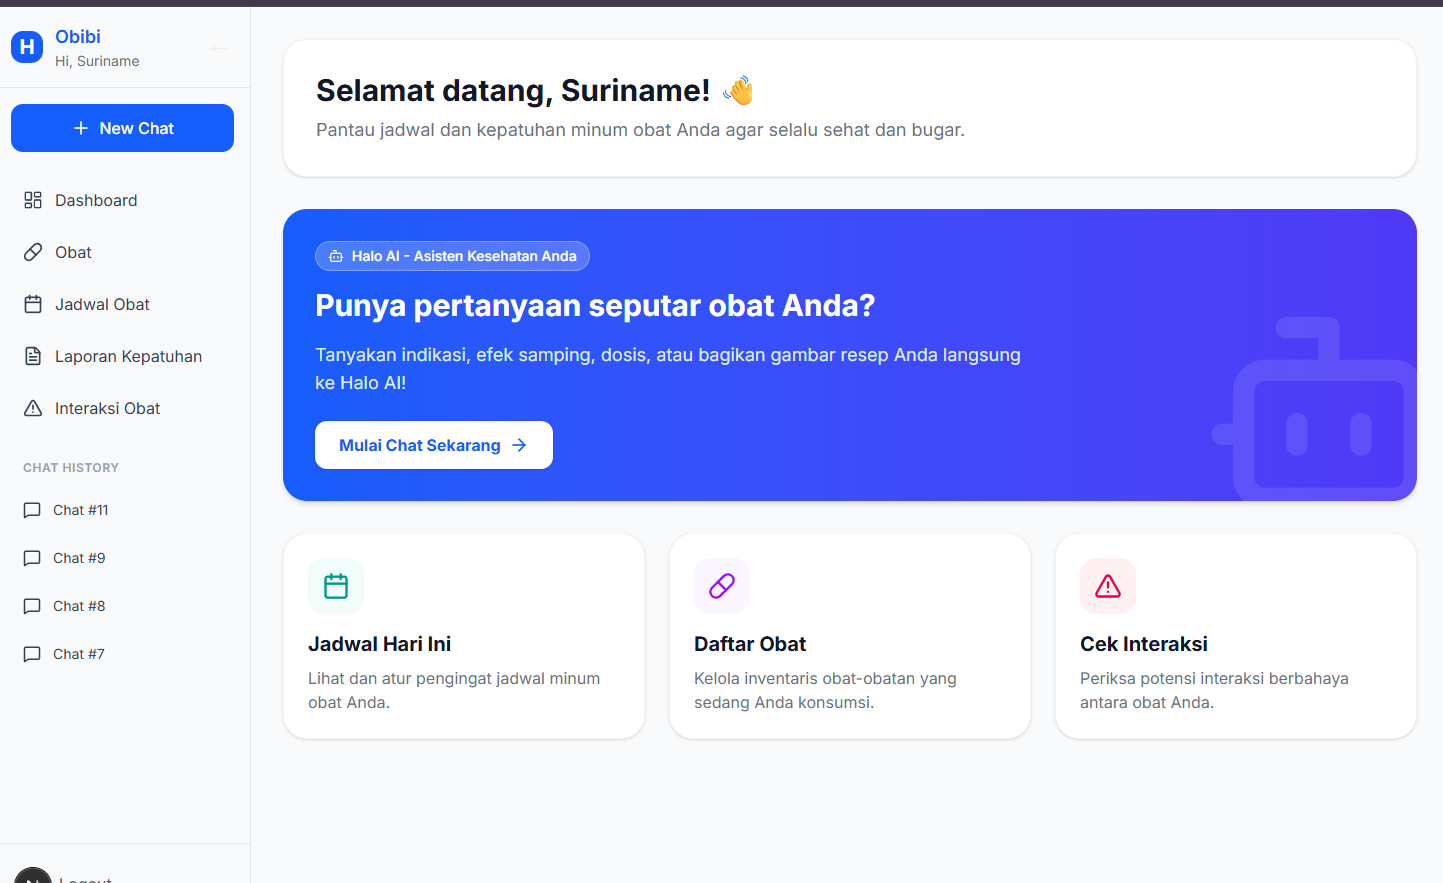
\includegraphics[width=0.8\textwidth]{loginberhasil.png}
  \caption{Screenshot Pelaksanaan Uji DUPL-LOGIN-01 (Login Sukses)}
  \label{fig:screenshot_register}
\end{figure}

\begin{figure}[H]
  \centering
  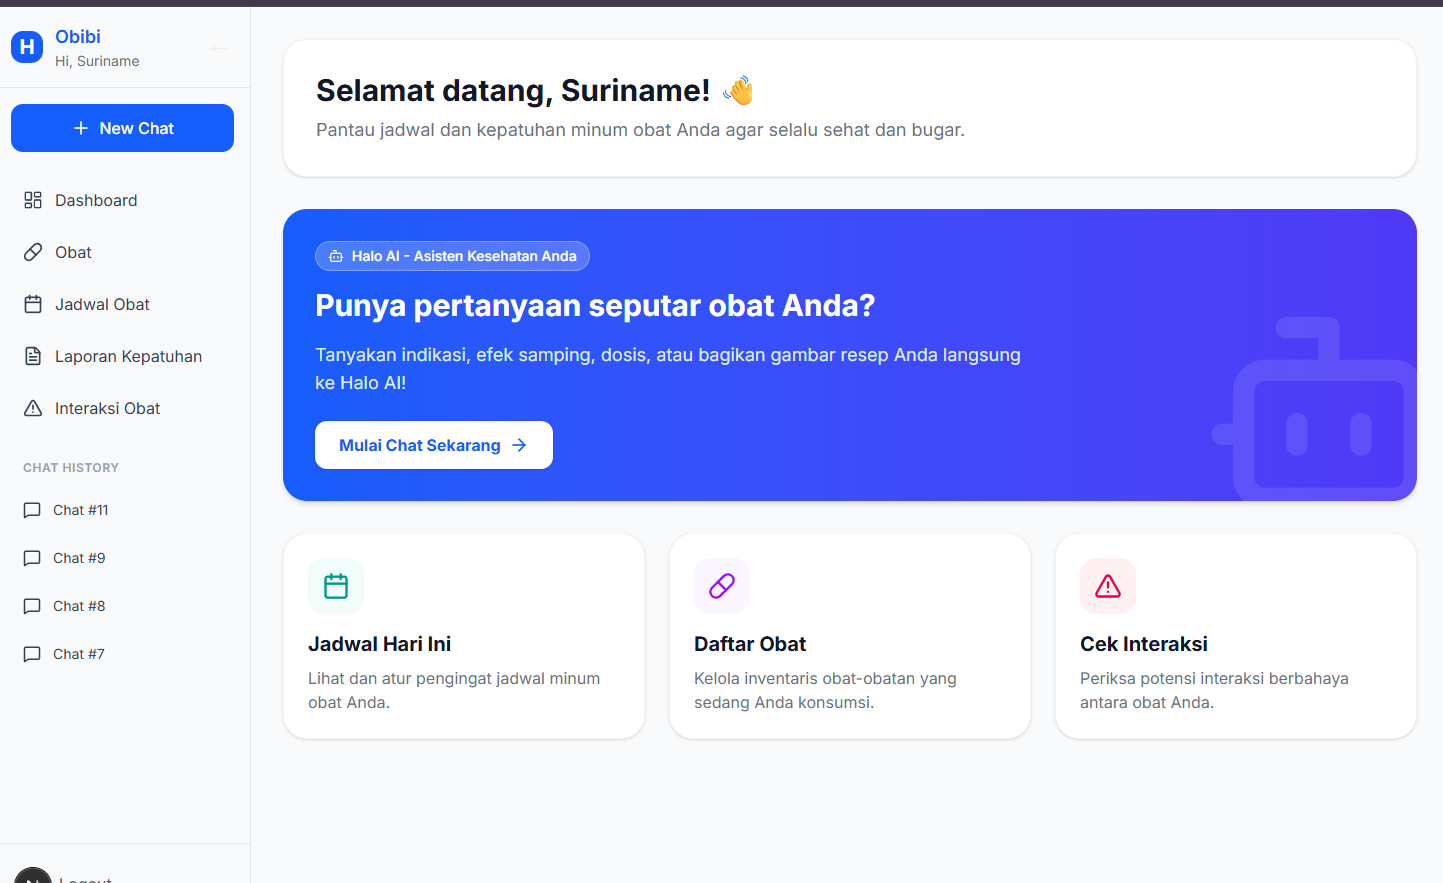
\includegraphics[width=0.8\textwidth]{registerberhasil.png}
  \caption{Screenshot Pelaksanaan Uji DUPL-REGISTER-01 (Register Sukses)}
  \label{fig:screenshot_register}
\end{figure}

\nopagebreak
\begin{figure}[H]
  \centering
  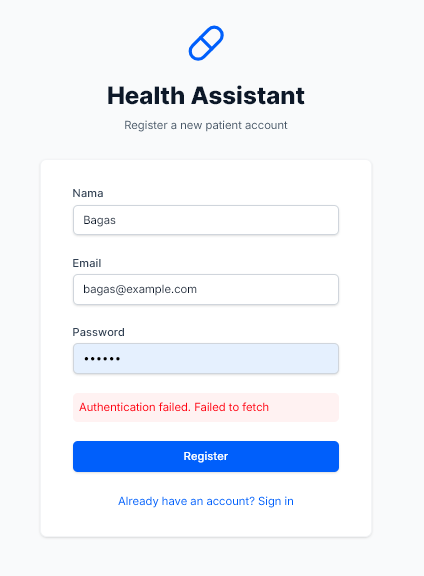
\includegraphics[width=0.8\textwidth]{regErrornointernet.png}
  \caption{Screenshot Pelaksanaan Uji DUPL-LOGIN-02 / DUPL-REGISTER-02 (Pesan Error Koneksi Terputus)}
  \label{fig:screenshot_login_error}
\end{figure}

\newpage
\begin{figure}[H]
  \centering
  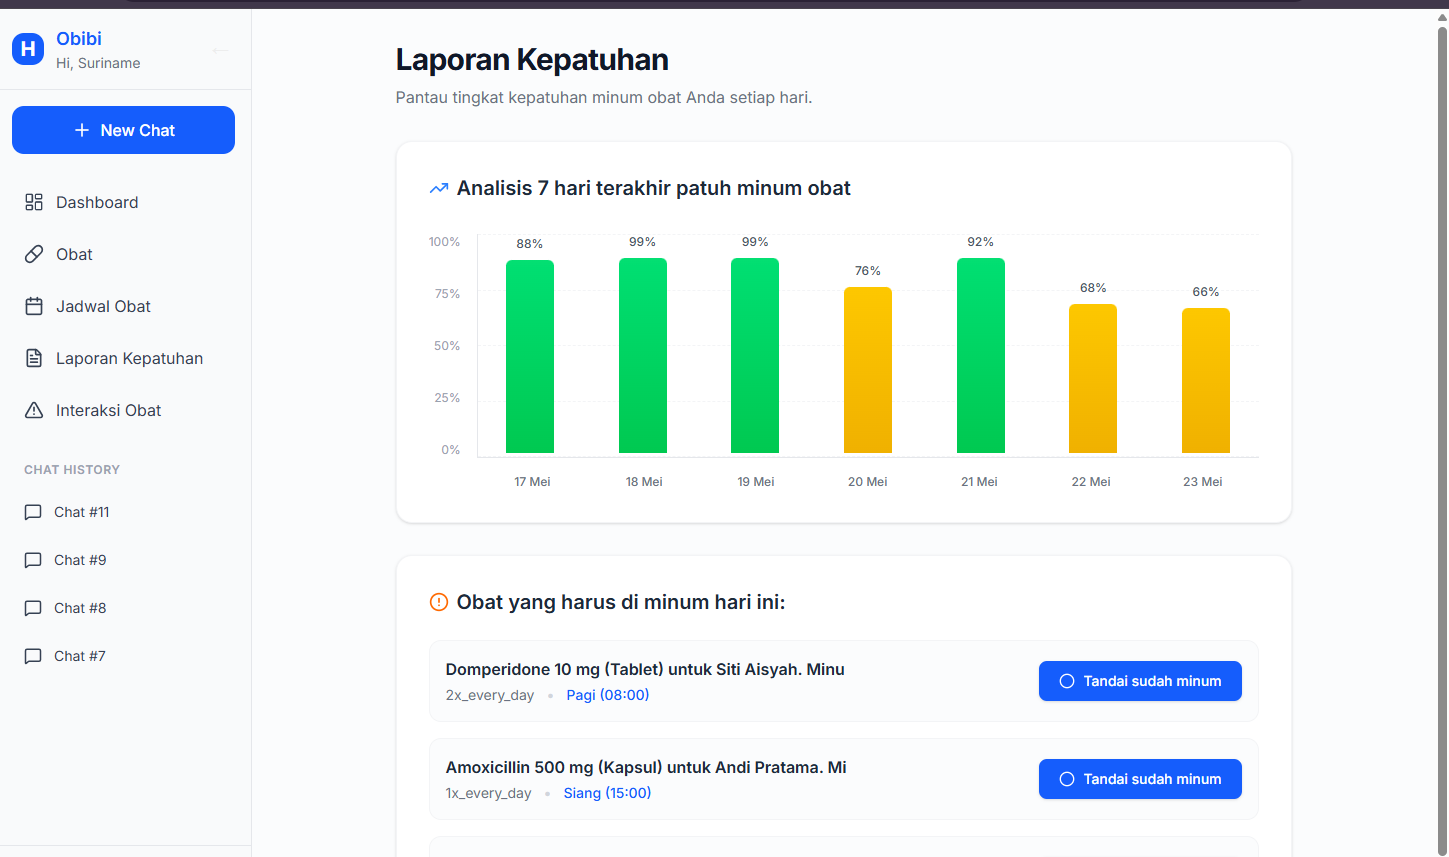
\includegraphics[width=0.8\textwidth]{laporankepatuhan.png}
  \caption{Screenshot Pelaksanaan Uji DUPL-INTERAKSI-01 (Hasil Analisis Interaksi Aspirin dan Ibuprofen)}
  \label{fig:screenshot_interaksi_obat}
\end{figure}

\nopagebreak
\begin{figure}[H]
  \centering
  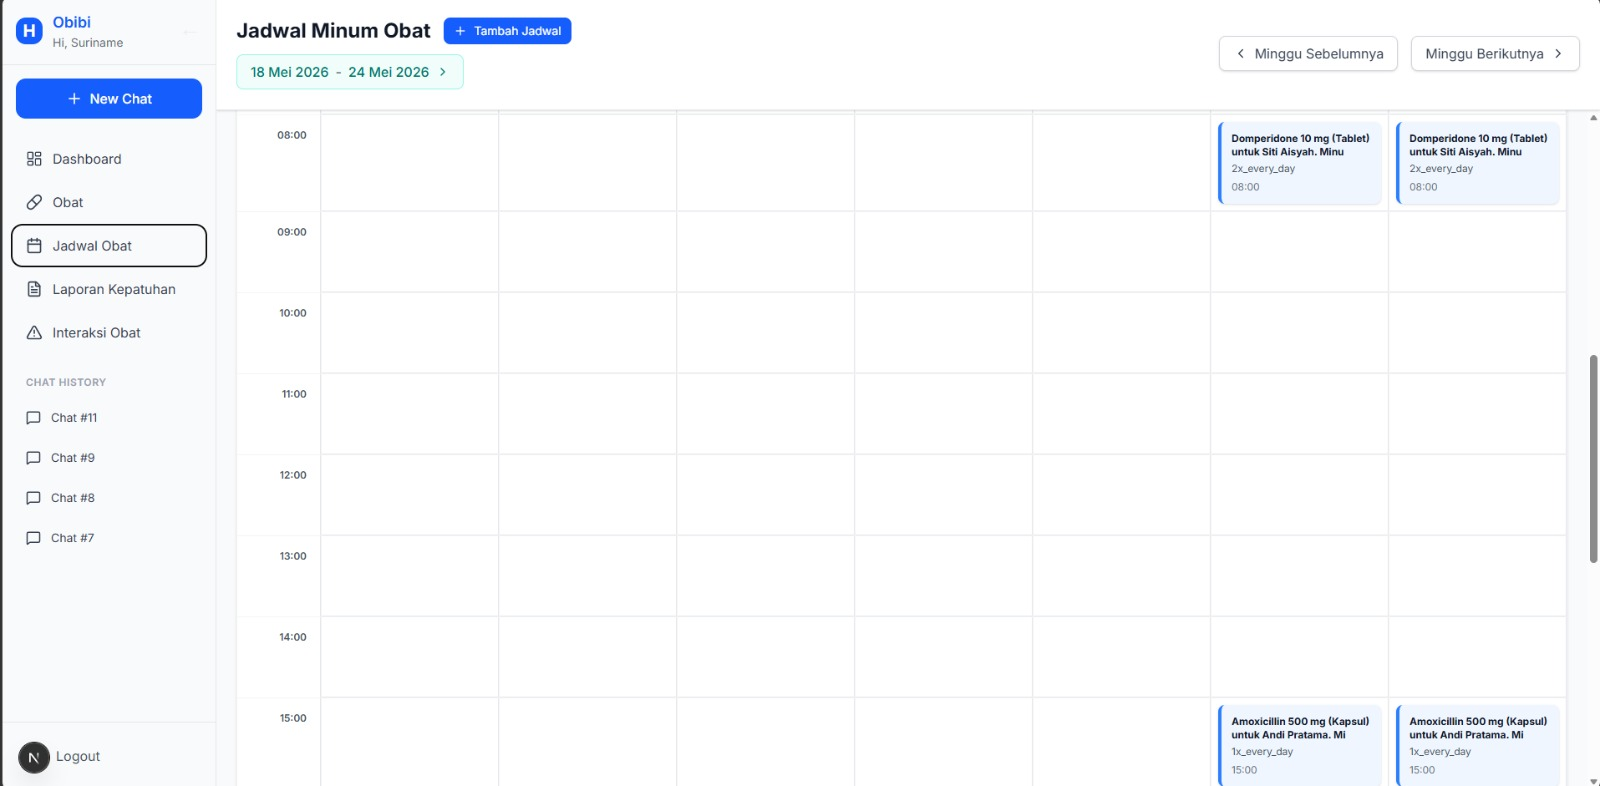
\includegraphics[width=0.8\textwidth]{jadwal_obat.jpeg}
  \caption{Screenshot Pelaksanaan Uji DUPL-JADWAL-01 (Input Batasan Waktu Pengingat Dosis Obat)}
  \label{fig:screenshot_tambah_jadwal}
\end{figure}

\vspace{1cm}
\begin{table}[h!]
  \centering
  \begin{tabular}{|p{5cm}|p{4cm}|p{4cm}|}
    \hline
    \textbf{Prodi Informatika -- Universitas Telkom}
      & \textbf{DUPL-xxx}
      & \textbf{Halaman \underline{\hspace{1cm}} dari \underline{\hspace{1cm}}} \\
    \hline
  \end{tabular}
\end{table}

\end{document}